\documentclass[fontsize=12pt,		% Font size
			   toc=listof,			% List of... into table of contents % listofnumbered
			   paper=A4,			% A4 paper
			   headinclude=true,	% Include header into type area calculation
			   footinclude=false,	% Don't include footer into type area calculation
			   headsepline=true,	% Separating line between header and text
			   footsepline=false,	% Separating line between footer and text
			   DIV=calc,			% Auomatically calculate DIV
			   %BCOR=15mm,			% Binding correction
			   %twosided=true,
			   %open=right
			  ]{scrartcl}

\usepackage[english,ngerman]{babel}
\usepackage[utf8]{inputenc}
\usepackage[T1]{fontenc}

\usepackage{lmodern}
\usepackage{microtype}

\usepackage{textcomp}				% Avoids conflicts between siunitx and microtype
\usepackage{siunitx}				% Allow for german decimals, e.g. 1,344 instead of 1.344 + other stuff

\usepackage{graphicx}
\usepackage{listings}
\usepackage{color}
\usepackage{hyperref}

% Autorenangabe
\newcommand\mychapter[2]{\chapter{#2}\vspace{-1.5em}\hspace{2.1em}\emph{#1}\vspace{1.5em}}
\newcommand\mysection[2]{\section{#2}\vspace{-0.9em}\hspace{2.1em}\emph{#1}\vspace{1.5em}}
\newcommand\mysubsection[2]{\subsection{#2}\vspace{-0.5em}\hspace{3.2em}\emph{#1}\vspace{1.3em}}

% ToDO

\newcommand\todo[1]{\footnote{\textcolor{red}{\textbf{#1}}}}

% PDF Metadaten

\pdfinfo{
 /Title (BlinkenTiles)
 /Author (Fabian Gärtner, Sarah Häfele, Alexander Scheurer, Linda Schey, Johannes Winter, Meike Zöckler)
}

\begin{document}


%%%%%%%%%%%%%%%%%%%%%%%%%%%%%%%%%%%%%%%%%
% University Assignment Title Page 
% LaTeX Template
% Version 1.0 (27/12/12)
%
% This template has been downloaded from:
% http://www.LaTeXTemplates.com
%
% Original author:
% WikiBooks (http://en.wikibooks.org/wiki/LaTeX/Title_Creation)
%
% License:
% CC BY-NC-SA 3.0 (http://creativecommons.org/licenses/by-nc-sa/3.0/)
% 
% Instructions for using this template:
% This title page is capable of being compiled as is. This is not useful for 
% including it in another document. To do this, you have two options: 
%
% 1) Copy/paste everything between \begin{document} and \end{document} 
% starting at \begin{titlepage} and paste this into another LaTeX file where you 
% want your title page.
% OR
% 2) Remove everything outside the \begin{titlepage} and \end{titlepage} and 
% move this file to the same directory as the LaTeX file you wish to add it to. 
% Then add \input{./title_page_1.tex} to your LaTeX file where you want your
% title page.
%
%%%%%%%%%%%%%%%%%%%%%%%%%%%%%%%%%%%%%%%%%

%----------------------------------------------------------------------------------------
%	PACKAGES AND OTHER DOCUMENT CONFIGURATIONS
%----------------------------------------------------------------------------------------

%\documentclass[12pt]{article}

%\begin{document}

\begin{titlepage}

\newcommand{\HRule}{\rule{\linewidth}{0.5mm}} % Defines a new command for the horizontal lines, change thickness here

\center % Center everything on the page
 
%----------------------------------------------------------------------------------------
%	HEADING SECTIONS
%----------------------------------------------------------------------------------------

\Large Hochschule Furtwangen - Fakultät Digitale Medien\\[0.5cm] % Name of your university/college
{\Large \bfseries Interaktionsdesign}\\[0.5cm] % Major heading such as course name
\large Wintersemester 2014/15\\[0.5cm] % Minor heading such as course title

%----------------------------------------------------------------------------------------
%	TITLE SECTION
%----------------------------------------------------------------------------------------

\HRule \\[0.2cm]
%{ \huge \bfseries BlinkenTiles}\\[0cm] % Title of your document

\includegraphics[width=0.5\textwidth]{images/logo_final}\\[-0.35cm]
\HRule \\[0.7cm]
 
%----------------------------------------------------------------------------------------
%	AUTHOR SECTION
%----------------------------------------------------------------------------------------

\begin{minipage}{0.55\textwidth}
\begin{flushleft} \large
%\emph{Authoren:}\\
Fabian Gärtner, MIM1\\
Sarah Häfele, MIM1\\
Alexander Scheurer, MIM1\\
Linda Schey, MIM2\\
Johannes Winter, DIM1\\
Maike Zöckler, DIM1\\

\end{flushleft}
\end{minipage}
~
\begin{minipage}{0.4\textwidth}
\begin{flushright} \large
%\emph{Supervisor:} \\
Prof. Patricia Stolz\\
Prof. Dr. Matthias Wölfel\\ % Supervisor's Name
\end{flushright}
\end{minipage}\\[2cm]

% If you don't want a supervisor, uncomment the two lines below and remove the section above
%\Large \emph{Author:}\\
%John \textsc{Smith}\\[3cm] % Your name

%----------------------------------------------------------------------------------------
%	DATE SECTION
%----------------------------------------------------------------------------------------

{\large \today}\\[3cm] % Date, change the \today to a set date if you want to be precise

%----------------------------------------------------------------------------------------
%	LOGO SECTION
%----------------------------------------------------------------------------------------

%\includegraphics{Logo}\\[1cm] % Include a department/university logo - this will require the graphicx package
 
%----------------------------------------------------------------------------------------

\vfill % Fill the rest of the page with whitespace

\end{titlepage}
%\end{document}

\section*{Abstract}
\section*{Abstract}
Die vorliegende Arbeit stellt die Dokumentation zur Konzeption und prototypischen Umsetzung von \emph{BlinkenTiles} dar. BlinkenTiles ist eine großflächige Installation, die es Personen erlaubt, durch eine auf den Boden projizierte Sound-Matrix und durch das Tracking einer Microsoft Kinect mit dem eigenen Körper Musik zu machen. Die Installation wurde im Rahmen der Veranstaltung \textit{Interaktionsdesign} in den Masterstudiengängen \textit{Design Interaktiver Medien} sowie \textit{Medieninformatik} an der Fakultät Digitale Medien der Hochschule Furtwangen im Wintersemester 2014/2015 unter der Betreuung von Frau Prof. Stolz und Herrn Prof. Dr. Wölfel entwickelt.

\tableofcontents
\clearpage

%Bitte im folgenden \includes{} nutzen!


\section{Grundidee}
\subsection{Ideenfindung}
\subsection{Zielsetzung}
\subsection{Werbebotschaft}
\subsection{Strategische Planung}

\section{Planung und Skizzierung}
\subsection{Zielgruppenanalyse}
\subsection{Tests}
\subsection{Technischer Aufbau}

\section{Umsetzung des Prototypen}
\subsection{Modell Aufbau}
\subsection{DMX-Scheinwerfer}
\subsection{Multimonitor Support}
\subsection{Tiles-Programmierung}
\subsection{Modi}
\subsection{Call to Action}
\mysubsection{Fabian Gärtner}{Personenerkennung mittels Microsoft Kinect}

Zur Erkennung von Personen auf dem Spielfeld mittels Microsoft Kinect konnten keine Standardfunktionen verwendet werden, da das Kinect-SDK den Einsatz der Kinect aus der Vogelperspektive nicht vorsieht. Stattdessen muss das von der Kinect aufgenommene Tiefenbild mittels Bildverarbeitungstechniken auf Personen bzw. verallgemeinert gesprochen auf Objektkonturen hin untersucht werden. In BlinkenTiles sind dafür die drei Klassen \enquote{KinectManager}, \enquote{BlobDetection} und \enquote{BlobDetectionThread} zuständig. Erstere fragt unter Anwendung des Kinect-SDKs von Microsoft das Tiefenbild (30 Bilder pro Sekunde mit einer Auflösung von 512 x 424 Pixel) und -- bei Bedarf -- das Farbbild (15 Bilder pro Sekunde mit einer Auflösung von 1920 x 1080 Pixel) der Kinect ab. Das Tiefenbild ist dabei ein zweidimensionales Array, das mit Werten zwischen 0 und 8000 die pro Pixel gemessene Tiefe in Millimeter angibt. Da sich die Farbkamera von der Tiefenkamera in Auflösung und Bildwinkel unterscheidet, müssen die Werte des Farbbildes, um beide Bilder übereinander legen zu können, mittels einer vom Kinect-SDK bereitgestellten Funktion umgerechnet werden. Auch diese Funktionalität und die Möglichkeit, Tiefenbilder in Form von Dateien abzuspeichern und für den Fall, dass die Kinect nicht angeschlossen ist, als Testdaten zu verwenden, stellt die Klasse bereit.

Die Weiterverarbeitung des Tiefenbildes und damit die eigentliche Bildverarbeitung findet in der Klasse \enquote{BlobDetectionThread} statt und wird zur Laufzeit in einem eigenen Thread ausgeführt. Dies war zu Beginn der Entwicklung noch notwendig, da die anfangs prozessorlastige Objekterkennung zu einer niedrigen Bildrate in der Hauptanwendung führte und damit auch Auswirkungen auf den Spielablauf und das Abspielen der Musik hatte. Dieser Prozess konnte im Verlauf der Entwicklung aber stetig optimiert werden, sodass die Bildverarbeitung auf eine Dauer von lediglich 12 Millisekunden pro Tiefenbild reduziert werden konnte. Mit etwas mehr als 80 Bildern pro Sekunde liegt die Objekterkennung damit bereits weit über der Bildrate der Kinect mit rund 30 Bildern pro Sekunde und kann ohne Verzögerung und in Echtzeit stattfinden. Die Auslagerung in einen eigenen Thread wurde aber beibehalten, sodass die Arbeitslast auch weiterhin gleichmäßig auf mehrere CPU-Kerne verteilt wird und mögliche Verzögerungen bei der Abfrage der Tiefenbilder keine Auswirkungen auf die Hauptanwendung und den Spielablauf haben.

Hauptsächlich für die Bildverarbeitung verwendet wird die kostenfreie Open-Source-Bibliothek OpenCV, die über den C-Sharp-Wrapper EmguCV angesteuert wird. OpenCV erlaubt die Anwendung von Algorithmen und grundlegenden mathematischen Operationen auf Matrizen und Bilder. Konkret wird bei BlinkenTiles zunächst das als Array vorliegende Bild gefiltert und normalisiert. Die Filterung arbeitet anhand vom Nutzer eingestellter Werte für minimale und maximale Tiefe. Alle Werte über und alle Werte unter diesen Vorgaben werden auf 0 gesetzt, sodass diese die Erkennung nicht weiter stören. In der Praxis kann damit ein stark reflektierender Boden herausgefiltert werden. Die anschließende Normalisierung hilft, den Kontrast des Tiefenbildes zu erhöhen und so die dann folgende Binarisierung des Bildes zu optimieren. Auf das binarisierte Bild wird letztlich die Konturerkennung von OpenCV angewendet, die Objekte ab einer bestimmten Größe erkennt und ein entsprechendes Konturrechteck zurückliefert. Dieses Rechteck kann anschließend mit den Feldern der Matrix abgeglichen werden und bei Überschneidungen zwischen Konturrechteck und einem Feld das Feld aktiviert werden. Jeder dieser Schritte ist vom Nutzer über eine im Folgenden näher erläuterte GUI separat darstellbar und konfigurierbar, um eine optimale Objekterkennung zu ermöglichen. Des Weiteren werden regelmäßig die einzelnen Schritte als Bilder herausgespeichert, sodass sie den Spielern über den Präsentationsbildschirm angezeigt werden können.

Die Klasse \enquote{BlobDetection} schließlich ist hauptsächlich für die Verwaltung der grafischen Benutzeroberfläche (GUI) der Bildverarbeitung und die Verwaltung der eben beschriebenen Klassen zuständig. Dieser Teil der GUI, wie er in Abbildung X auf Seite X dargestellt ist, nimmt die linke Hälfte der gesamten GUI von BlinkenTiles ein und erstreckt sich damit über einen Monitor. Die GUI stellt das Tiefenbild in seiner ursprünglichen Form oder nach einem der zuvor beschriebenen Verarbeitungsschritte, bspw. in binarisierter Form oder mit farbigen Konturrechtecken um erkannte Objekte, dar. Des Weiteren erlaubt die GUI über eine Reihe von Slidern die Einstellung von Filterwerten, Spielfeld- und Feldergröße sowie Spielfeldposition. Ebenso kann ein Raster über dem Tiefenbild dargestellt werden, bei dem alle aktivieren Felder, also alle Felder auf denen Personen erkannt wurden, farbig markiert sind. Um dieses Raster dem vom Beamer erzeugten Spielfeld anzupassen, also um Beamer und Kinect zu synchronisieren, besteht die Möglichkeit eine Überlagerung von Farb- und Tiefenbild anzuzeigen, die dann die Anpassung der Größe und Ausrichtung des Rasters auf dem Tiefenbild mittels der Slider erlaubt. Alle Einstellungen können auch zuvor über die externe Konfigurationsdatei geladen werden.

\subsubsection{Aufgetretene Probleme}

Am Tag der Medien zeigte sich, dass die Tische, auf denen u.\,a. die LED-Scheinwerfer standen, aufgrund ihrer hellen Oberfläche nicht aus dem Tiefenbild herausgefiltert werden konnten und daher ebenfalls als Objekte erkannt wurden. Dies führte dazu, dass Personen, die auf einem der Felder in der Nähe der Tische standen, zusammen mit den Tischen als ein großes Objekt erkannt und dadurch gelegentlich zu viele Felder gleichzeitig aktiviert wurden. Beheben ließe sich das Problem, indem das Tiefenbild vor der weiteren Verarbeitung auf den relevanten Bereich, also auf Spielfeldgröße zugeschnitten wird. Auch hierfür könnten entsprechende Regler in die GUI integriert werden, sodass der Zuschnitt manuell und je nach Bedarf eingestellt werden kann.

Ein weiteres Problem ist die Perspektive, vor allem dann, wenn die Kinect nicht mittig über dem Spielfeld hängt. So funktioniert die Erkennung von Personen, die sich direkt unter der Kinect befinden zwar tadellos, je weiter eine Person aber von der Kinect entfernt ist, desto mehr Felder deckt sie aufgrund der schrägen Aufsicht gleichzeitig ab. Eine kurzfristige Lösung am Tag der Medien war es, die Felder in der Anwendung größer als in der Realität einzustellen. Des Weiteren wird bereits nicht das ganze Feld auf Überschneidungen mit Konturen überprüft, sondern lediglich ein kleinerer (ebenfalls einstellbarer) Bereich in der Mitte der Felder. Um das Problem aber besser zu lösen, wäre entweder eine zweite Kinect oder eine perspektivisch korrekte Berechnung und ein unsymmetrisches Raster notwendig. So könnten bspw. die Felder des Rasters in den Randbereichen vergrößert oder die Tiefenfilterung zu den Rändern hin verstärkt werden, sodass in diesen Bereichen nur noch die Beine von Personen für die Überschneidung relevant sind, nicht aber der Kopf, der möglicherweise ein anderes Felder überdeckt. Welche Methode sich hier am besten eignet, müsste durch weitere Tests herausgefunden werden.

Störend war auch, dass die Einstellungen zwar wie beschrieben aus einer Konfigurationsdatei geladen werden können, die Werte aber momentan noch per Hand eingetragen werden müssen. Interessant neben einem Button zum Speichern der Einstellungen könnte für eine solche Installation daher auch eine automatische Kalibrierung sein, um bei einem Neustart die manuelle Neukonfiguration zu vermeiden. Technisch ließe sich das über ein vom Beamer dargestelltes Testmuster lösen, das von der Bildverarbeitung erkannt wird und das Raster entsprechend dimensionieren und positionieren lässt. Auch die optimalen Werte für die Filterung könnten so automatisiert ermittelt werden.


\newpage

\begin{figure}[htbp] 
  \centering
     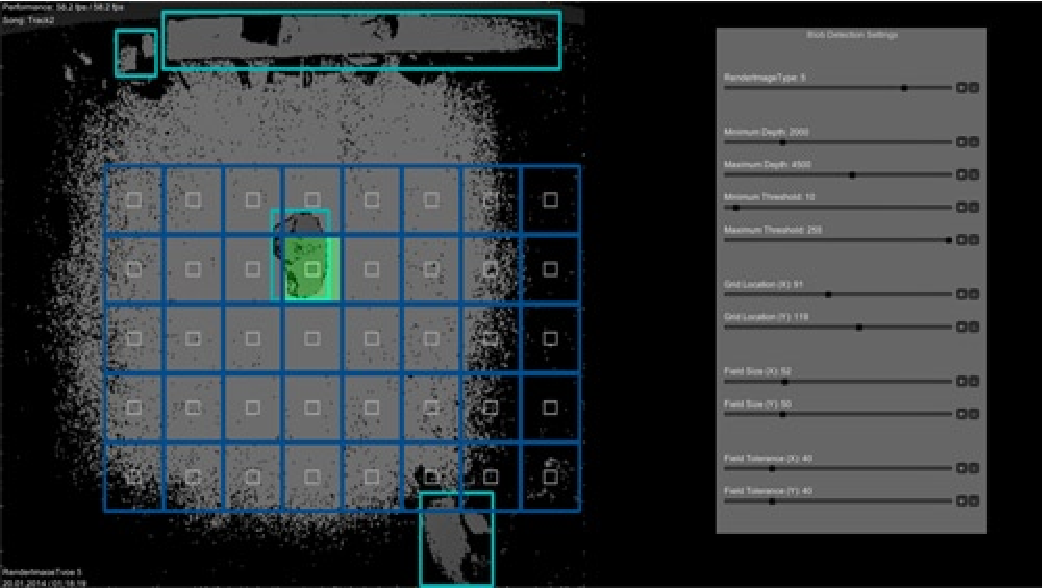
\includegraphics[width=0.9\textwidth]{images/Blob}
  \caption{Schneiden der Spuren in Ableton Live}
  \label{fig:blob}
\end{figure}\todo{caption}

\subsection{Audiogestaltung und Inspiration}
Das Konzept der Installation beruht auf einem klassischen Step-Sequenzer. Solche Sequenzer steuern die Klangerzeugung eines Synthesizers dahingehend, dass sowohl Rhythmus als auch Tonhöhe programmiert werden können. Der Name bezieht sich dabei auf die einzelnen „Steps“ die mit Tönen belegt werden können. Klassische analoge Step-Sequenzer wie der Roland TB 303 bieten 16 Schritte an, womit also pro Durchlauf 16 Töne gespielt werden können. Somit entspricht jeder Schritt einer 16tel Note eines Taktes. Es ist hervorzuheben, dass bei einem Step-Sequenzer die Noteneingabe nicht unmittelbar zu einer Klangerzeugung führt. Stattdessen tastet ein Impuls nacheinander alle „Steps“ ab und übermittelt die Daten an den Klangerzeuger. Nachdem der Impuls einmal durchgelaufen ist, beginnt der er wieder bei dem ersten Step. Dadurch entstehen repetitive Tonfolgen, sogenannte Loops. Step-Sequenzer haben gerade aufgrund dieser Beschränkung zahlreiche Genre wie Acid House, Electronic Body Music und Drum and Bass entscheidend geprägt.

Das Konzept der Installation weicht in mehreren Punkten vom klassischen Step-Sequenzer ab. Zum Einen gibt es statt 16 Schritten nur 8. Außerdem ist die Tonauswahl auf 5 Tonhöhen pro Schritt begrenzt. Des Weiteren wird ist ein Ton nur so lange aktiviert, wie auch eine Person auf dem entsprechenden Feld steht. Das musikalische Konzept berücksichtigt diese Einschränkungen. Da nur 5 Töne gespielt werden können und auch nur 8 Steps zur Verfügung stehen, wird ein Backing Track benötigt, der eine harmonische Grundlage für das Spiel des Instrumentes bietet.

Anspruch der Installation war es aber weniger ein komplexes Instrument zu bieten, viel mehr eine musikalische Spielwiese. Aus diesem Grund liegt die Entscheidung nahe, sich die technischen Beschränkungen zu Nutze zu machen. Es wurde also auf eine Skala zurückgegriffen, die einerseits nur 5 Töne hat und andererseits keine Halbtonschritte aufweist: die Anhemitonische Pentatonik. Der Vorteil liegt darin, dass keine kleinen Sekunden und Tritoni gespielt werden können, die für unsere Hörgewohnheiten „unrein“ klingen. Durch diese Maßnahme wurde also sichergestellt, dass unabhängig von Menge und Position der Benutzer ein recht harmonisches Gesamtbild entsteht, auch wenn dadurch auf die Leittonwirkung einer Diatonik oder Hemitonischen Pentatonik verzichtet werden muss. Außerdem war der Tonumfang natürlich auf eine Oktave beschränkt, mehr als 5 Tonhöhen hätten das musikalische Ergebnis interessanter gestaltet aber auch die Nutzerfreundlichkeit eingeschränkt. Da die Installation in erster Linie intuitiv bedienbar sein sollte, wurde der Tonumfang nicht weiter ausgebaut.

Für den experimentellen Modus der Installation wurden drei Backing Tracks mit jeweils 5 zugehörigen Tonhöhen vorproduziert. Der durchlaufende Impuls wurde auf die Geschwindigkeit des entsprechenden Backing Tracks angepasst und die zugehörigen Töne auf die Felder gemappt. Da der Klangerzeuger kein Synthesizer sondern ein Sampler war, mussten die Einzeltöne im Voraus synthetisiert und gerendert werden. Grundsätzlich wurden eher sphärische Klänge mit langem Nachhall (entweder Reverb oder Hüllkurvengenerator) eingesetzt, da die Benutzer der Installation keinen Einfluss auf die Länge des Tons hatten. In Hüllkurvenparametern gesprochen musste also der Attack deutlich hörbar sein um ein auditives Feedback zu geben, die Sustainlautstärke musste relativ schnell erreicht werden und wesentlich leiser als der Attack sein, damit sich bei mehreren Personen die Sounds nicht zu stark überdeckten. Dadurch wurden relativ perkussive Klänge erzeugt, die durch den Nachhall eine gewisse Stetigkeit erreichten. Die Backing Tracks bildeten das rhythmische und harmonische Grundgerüst und wurden ebenfalls im Voraus produziert und gerendert. Dabei wurde Wert darauf gelegt, zwar eine harmonische Orientierung zu bieten, der Backing Track sollte jedoch keine komplexe harmonische Struktur aufweisen. In den Backing Tracks wurde also ebenfalls weitgehend auf die oben erwähnte Pentatonik zurückgegriffen, um aber ein wenig musikalische Spannung zu kreieren, wurden an ausgewählten Stellen auch Töne aus diatonischen Skalen verwendet.

Für den Challenge Modus wurden ebenfalls drei Backing Tracks und passende Töne vorproduziert, da jedoch die technischen und konzeptionellen Bedingungen andere waren, soll darauf noch näher eingegangen werden. Das Ziel des Challenge Modus ist es, mit der Installation bekannte Lieder nachzuspielen, ähnlich wie bei Guitar Hero. Problematisch ist jedoch, dass die Reaktionsgeschwindigkeit der Benutzer nicht so schnell ist wie es eigentlich nötig wäre. Das größte Hindernis ist jedoch, dass die Nutzer die Installation verlassen müssen, wenn sie keinen Ton spielen wollen. Sobald sie auf irgendeinem Feld stehen und der Impuls dieses erreicht wird der Ton getriggert, auch wenn er falsch ist. Anders gesagt: Die Zustände der Nutzer auf dem Spielfeld sind analog, benötigt wären aber digitale Zustände, an oder aus. Aus diesem Grund mussten Songs gefunden werden, die einerseits recht bekannt sind, ein minimales Tonspektrum aufweisen und langsam genug sind um mit der Installation spielbar zu sein. Die Entscheidung fiel auf „Smoke on the water“ von Deep Purple, „Paint it black“ von den Rolling Stones und “One” von Swedish House Mafia.

Die Ausschnitte der Lieder die benutzt werden sollten, wurden zunächst nachgespielt und aufgenommen. Dabei war es wichtig, hervorstechende Klangeigenschaften der Originale zu berücksichtigen um den Wiedererkennungswert nicht zu verlieren. Bei „Smoke on the water“ wurde beispielsweise ein bekannter britischer Röhrenverstärker mit vorgeschaltetem Overdrive verwendet. Nachdem alle Einzelspuren aufgenommen waren musste bestimmt werden, welche Spuren den Backing Track bildeten und welche Spur von den Nutzern gespielt werden sollte. Der Backing Track wurde dann ohne die entsprechende Spur gerendert. Die Spur die der Nutzer spielen sollte, musste nun in kleine Samples geschnitten werden um auf die verschiedenen Felder aufgeteilt werden zu können.

\begin{figure}[htbp] 
  \centering
     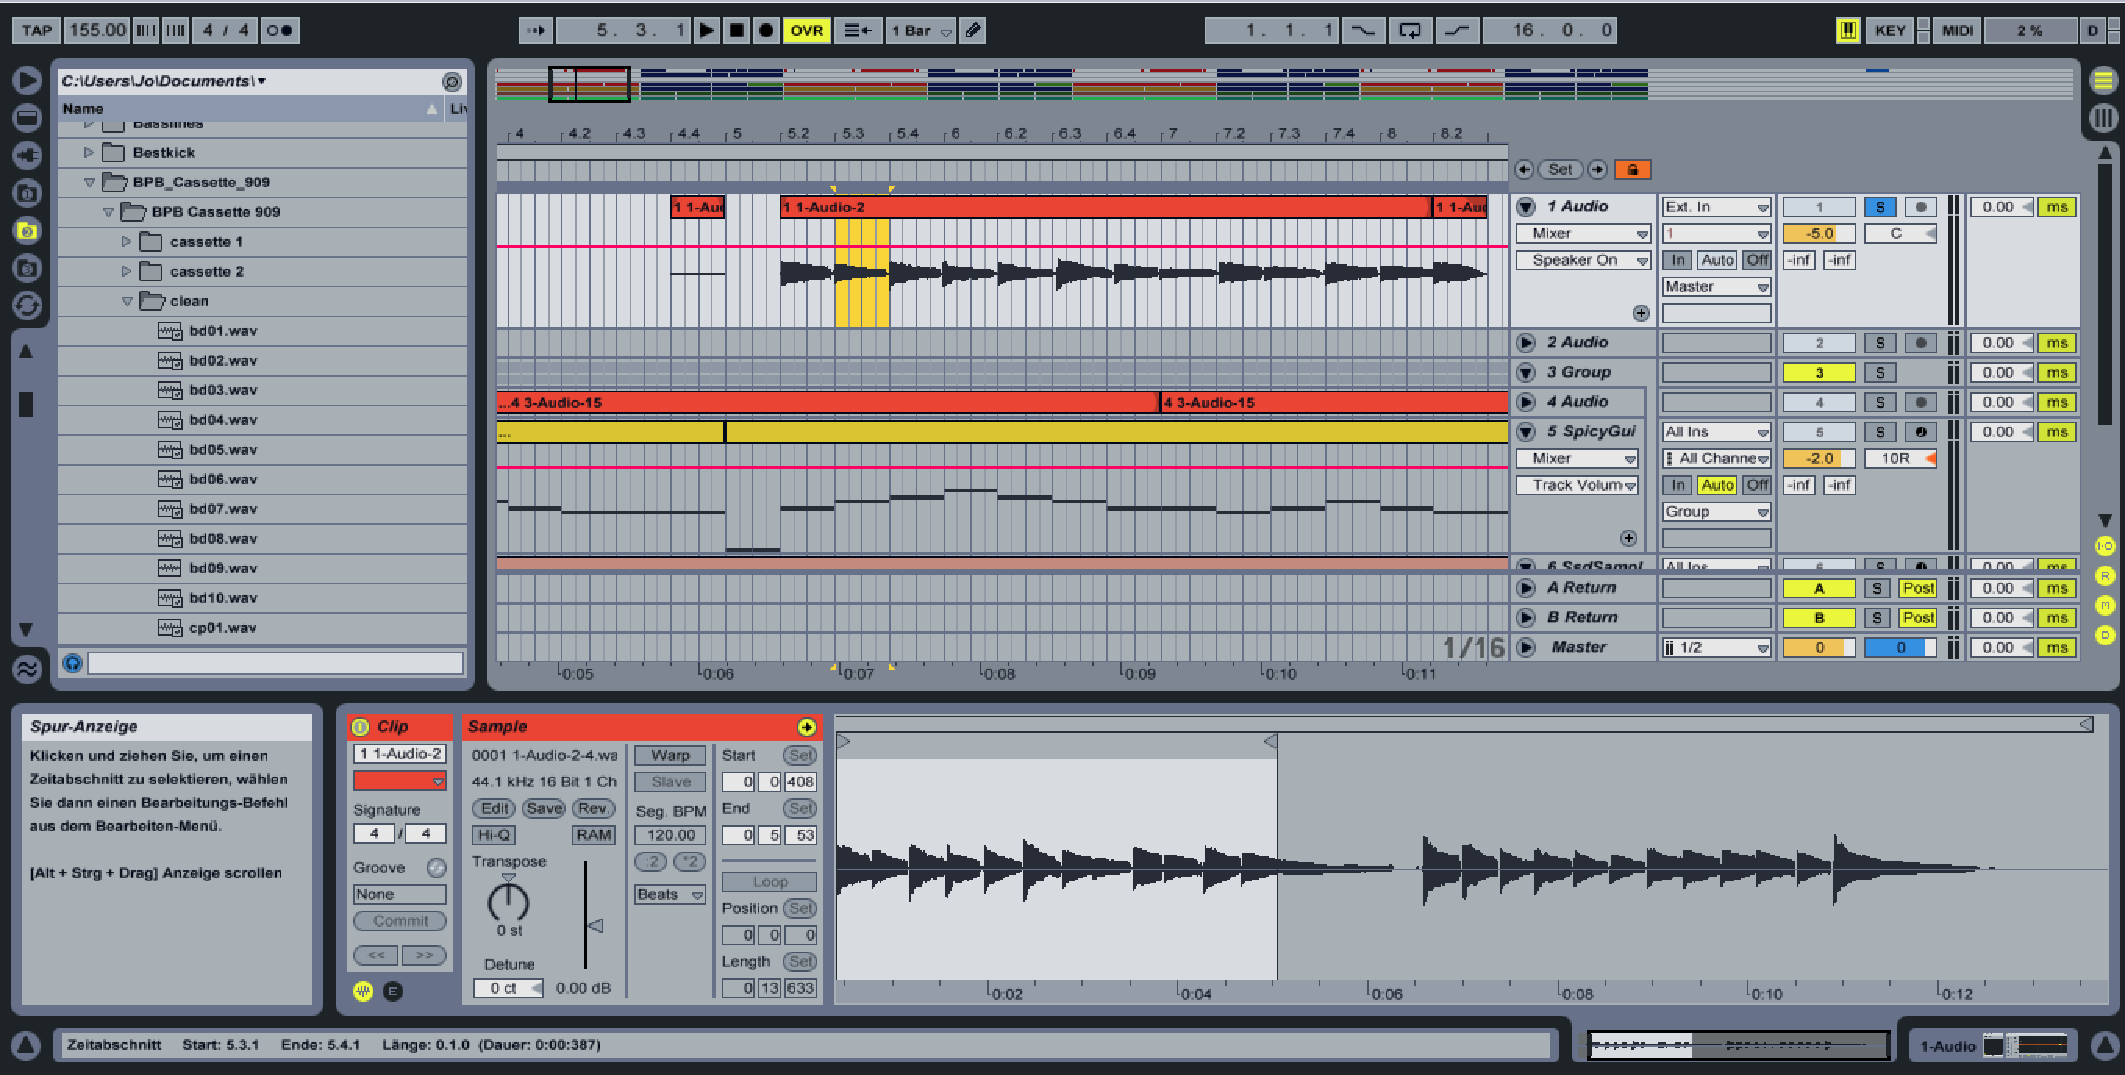
\includegraphics[width=0.9\textwidth]{images/Musikkonzeption}
  \caption{Schneiden der Spuren in Ableton Live}
  \label{fig:audio1}
\end{figure}

Dabei ergaben sich in einigen Fällen Probleme bezüglich der Tonlänge. Da die Schritte des Step-Sequenzers immer auf einen bestimmten Rhythmuswert quantisiert waren, zum Beispiel 8tel oder 16tel Noten, mussten hinsichtlich Synkopen oft Kompromisse eingegangen werden. Bei „One“ führte dies dazu, dass der Impuls so schnell war, dass das Lied damit praktisch unspielbar wurde. Für den Challenge Modus erwies sich damit das Konzept der Soundmatrix insgesamt als relativ ungeeignet, während im experimentellen Modus musikalisch interessante Ergebnisse erreicht wurden.

\section{Tag der Medien}
\subsection{kleiner Bericht mit Fotos}
\subsection{Praxiserfahrungen}

\section{Showreel}
\section{Fazit, mögl. Weiterentwicklungsmöglichkeiten}

\end{document}